% ===========================================================================
% fig_model_network_tikz.tex
% Diagrama estructural del modelo: red de logistica inversa a tres echelons
% (edificios -> hubs -> plantas) con apertura binaria irreversible y_{kt}.
% Compilar standalone, o copiar el entorno tikzpicture dentro del manuscrito
% (requiere \usepackage{tikz} y las librerias listadas abajo en el preambulo).
% ===========================================================================
\documentclass[tikz,border=6pt]{standalone}
\usetikzlibrary{positioning,arrows.meta,shapes.geometric,fit,backgrounds,calc}

\begin{document}
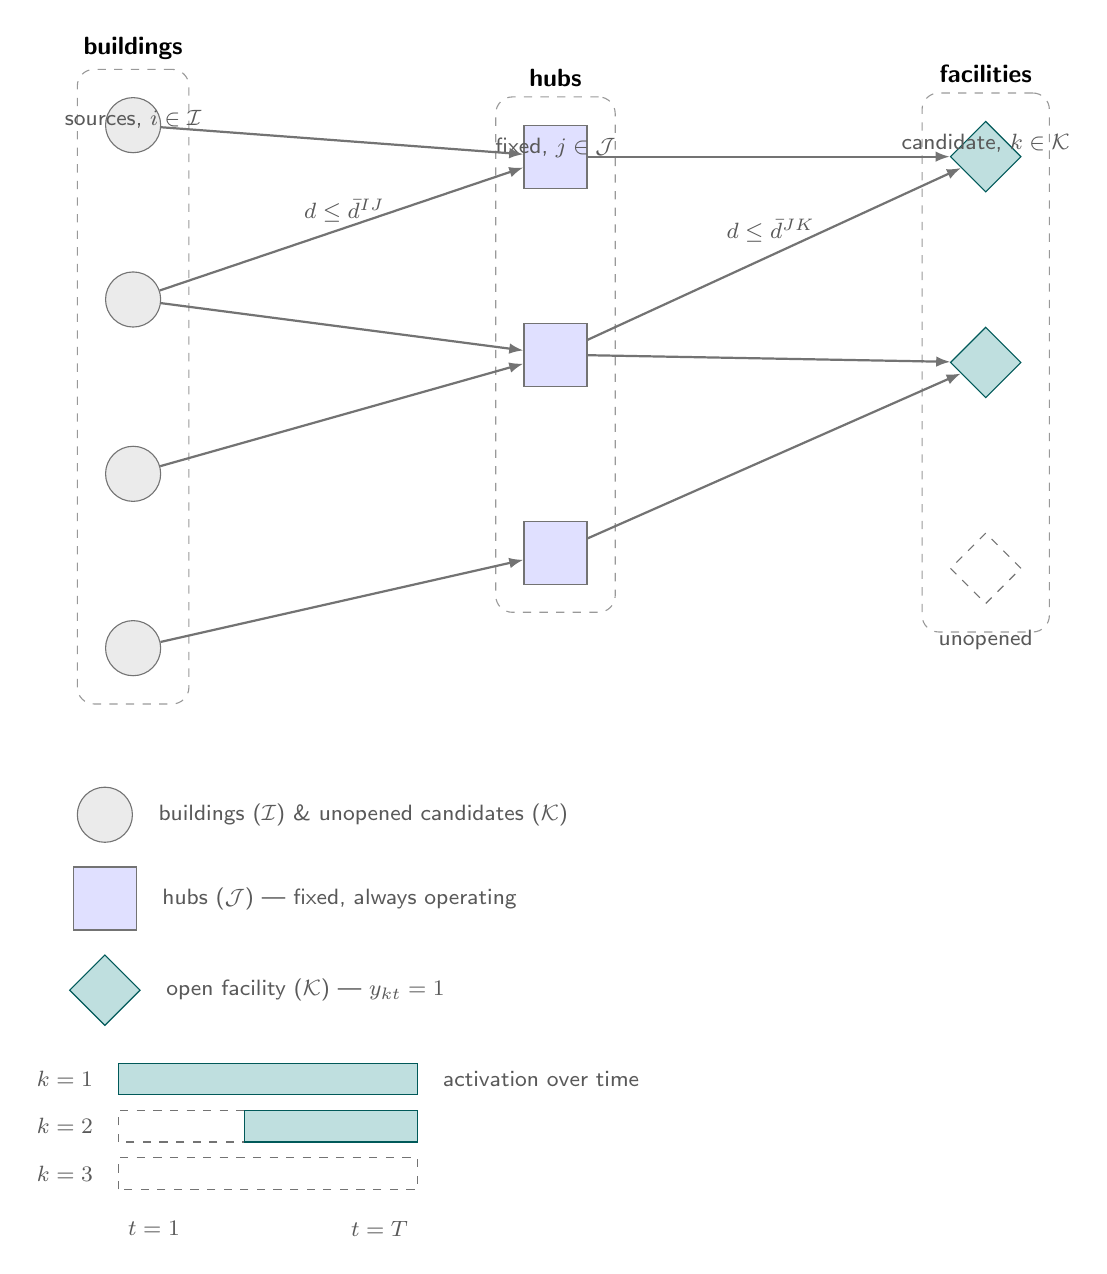
\begin{tikzpicture}[
  >={Latex[length=2mm,width=1.4mm]},
  font=\sffamily\small,
  build/.style ={circle,   draw=black!55, fill=black!8,   minimum size=7mm, inner sep=0pt},
  hub/.style   ={rectangle,draw=black!55, fill=blue!12,   minimum size=8mm, inner sep=0pt},
  facopen/.style ={diamond,draw=teal!70!black, fill=teal!25, minimum size=9mm, inner sep=0pt},
  facshut/.style ={diamond,draw=black!55, fill=none, dashed, minimum size=9mm, inner sep=0pt},
  grp/.style   ={draw=black!40, dashed, rounded corners=6pt, inner sep=10pt},
  lbl/.style   ={font=\sffamily\footnotesize, text=black!65},
  arc/.style   ={-{Latex[length=1.8mm]}, black!55, thick},
  node distance=15mm and 46mm
]

% ---- Column I: buildings (waste sources, exogenous) -----------------------
\node[build] (i1) {};
\node[build,below=of i1] (i2) {};
\node[build,below=of i2] (i3) {};
\node[build,below=of i3] (i4) {};

% ---- Column J: hubs (fixed, no activation variable) ------------------------
\node[hub, right=of i1, yshift=-4mm] (j1) {};
\node[hub, below=17mm of j1] (j2) {};
\node[hub, below=17mm of j2] (j3) {};

% ---- Column K: candidate facilities (binary y_{kt}) -------------------------
\node[facopen, right=of j1] (k1) {};
\node[facopen, below=17mm of k1] (k2) {};
\node[facshut, below=17mm of k2] (k3) {};

% ---- Group frames + headers -------------------------------------------------
\node[grp, fit=(i1)(i4), label={[lbl,font=\sffamily\bfseries\small,text=black]above:buildings}] (fitI) {};
\node[grp, fit=(j1)(j3), label={[lbl,font=\sffamily\bfseries\small,text=black]above:hubs}] (fitJ) {};
\node[grp, fit=(k1)(k3), label={[lbl,font=\sffamily\bfseries\small,text=black]above:facilities}] (fitK) {};

\node[lbl, below=1mm of fitI.north, yshift=-3mm] {sources, $i\in\mathcal{I}$};
\node[lbl, below=1mm of fitJ.north, yshift=-3mm] {fixed, $j\in\mathcal{J}$};
\node[lbl, below=1mm of fitK.north, yshift=-3mm] {candidate, $k\in\mathcal{K}$};

% ---- Admissible arcs (only within the distance threshold) ------------------
\draw[arc] (i1) -- (j1);
\draw[arc] (i2) -- (j1);
\draw[arc] (i2) -- (j2);
\draw[arc] (i3) -- (j2);
\draw[arc] (i4) -- (j3);

\draw[arc] (j1) -- (k1);
\draw[arc] (j2) -- (k1);
\draw[arc] (j2) -- (k2);
\draw[arc] (j3) -- (k2);

\node[lbl, above=1mm of $(i1)!0.5!(j2)$] {$d \le \bar d^{IJ}$};
\node[lbl, above=1mm of $(j1)!0.5!(k2)$] {$d \le \bar d^{JK}$};

\node[lbl, below=2mm of k3] {unopened};

% ---- Legend ------------------------------------------------------------------
\begin{scope}[shift={($(fitI.south west)+(0,-14mm)$)}]
  \node[build, anchor=west] (lg1) {};
  \node[lbl, right=2mm of lg1] {buildings ($\mathcal I$) \& unopened candidates ($\mathcal K$)};
  \node[hub, anchor=west, below=3mm of lg1] (lg2) {};
  \node[lbl, right=2mm of lg2] {hubs ($\mathcal J$) --- fixed, always operating};
  \node[facopen, anchor=west, below=3mm of lg2] (lg3) {};
  \node[lbl, right=2mm of lg3] {open facility ($\mathcal K$) --- $y_{kt}=1$};
\end{scope}

% ---- Activation timeline (irreversibility of y_{kt}) ------------------------
\begin{scope}[shift={($(lg3.south west)+(2mm,-9mm)$)}]
  \node[lbl, anchor=east] at (0,0)         {$k=1$};
  \node[lbl, anchor=east] at (0,-6mm)      {$k=2$};
  \node[lbl, anchor=east] at (0,-12mm)     {$k=3$};

  \fill[teal!25] (2mm,-2mm) rectangle ++(38mm,4mm);
  \draw[teal!70!black] (2mm,-2mm) rectangle ++(38mm,4mm);

  \draw[black!55,dashed] (2mm,-8mm) rectangle ++(16mm,4mm);
  \fill[teal!25] (18mm,-8mm) rectangle ++(22mm,4mm);
  \draw[teal!70!black] (18mm,-8mm) rectangle ++(22mm,4mm);

  \draw[black!55,dashed] (2mm,-14mm) rectangle ++(38mm,4mm);

  \node[lbl] at (2mm,-19mm) [anchor=west] {$t=1$};
  \node[lbl] at (40mm,-19mm) [anchor=east] {$t=T$};
  \node[lbl, anchor=west] at (42mm,0) {activation over time};
\end{scope}

\end{tikzpicture}
\end{document}
